% !TeX root = q1.tex
\subsection{Sizing and Layout}

The DroneStark drone presented in the market survey (shown in figure \ref{fig:sfig-q1-ms-ds}) is explored here. Some parts are not actually those that belong to the drone, but an approximate substitute is chosen.

\subsubsection*{Components}

The components that make up the system are described in paragraphs and images below

\paragraph*{Body frame}
The drone needs a body on which everything can rest. This is core mechanical design and has an assembly which can house all components of the drone (described hereon). The frame design of the DroneStark OctaGlide is shown in figure \ref{fig:sfig-szl-body-frame}. The body provides a nice $240\,mm$ by $240\,mm$ unit (height of approx. $165\,mm$) where all the electronics and the primary battery is housed.

\paragraph*{Dimensional specifications}
The drone is foldable, thanks to the body frame allowing it and the propellers themselves folding. The final structure, \emph{when folded} is $712\,mm$ in height, and the length and breadth is $640\,mm$. This makes it easy to transport. When \emph{fully extended} (ready to fly), the drone has $730\,mm$ height, with the total length and breadth being approximately $1688\,mm$. These are box dimensions of the drone. The body frame specifications can be found in figure \ref{fig:szl-body-specs}.

\begin{figure}[ht]
    \centering
    \begin{subfigure}[b]{0.3\textwidth}
        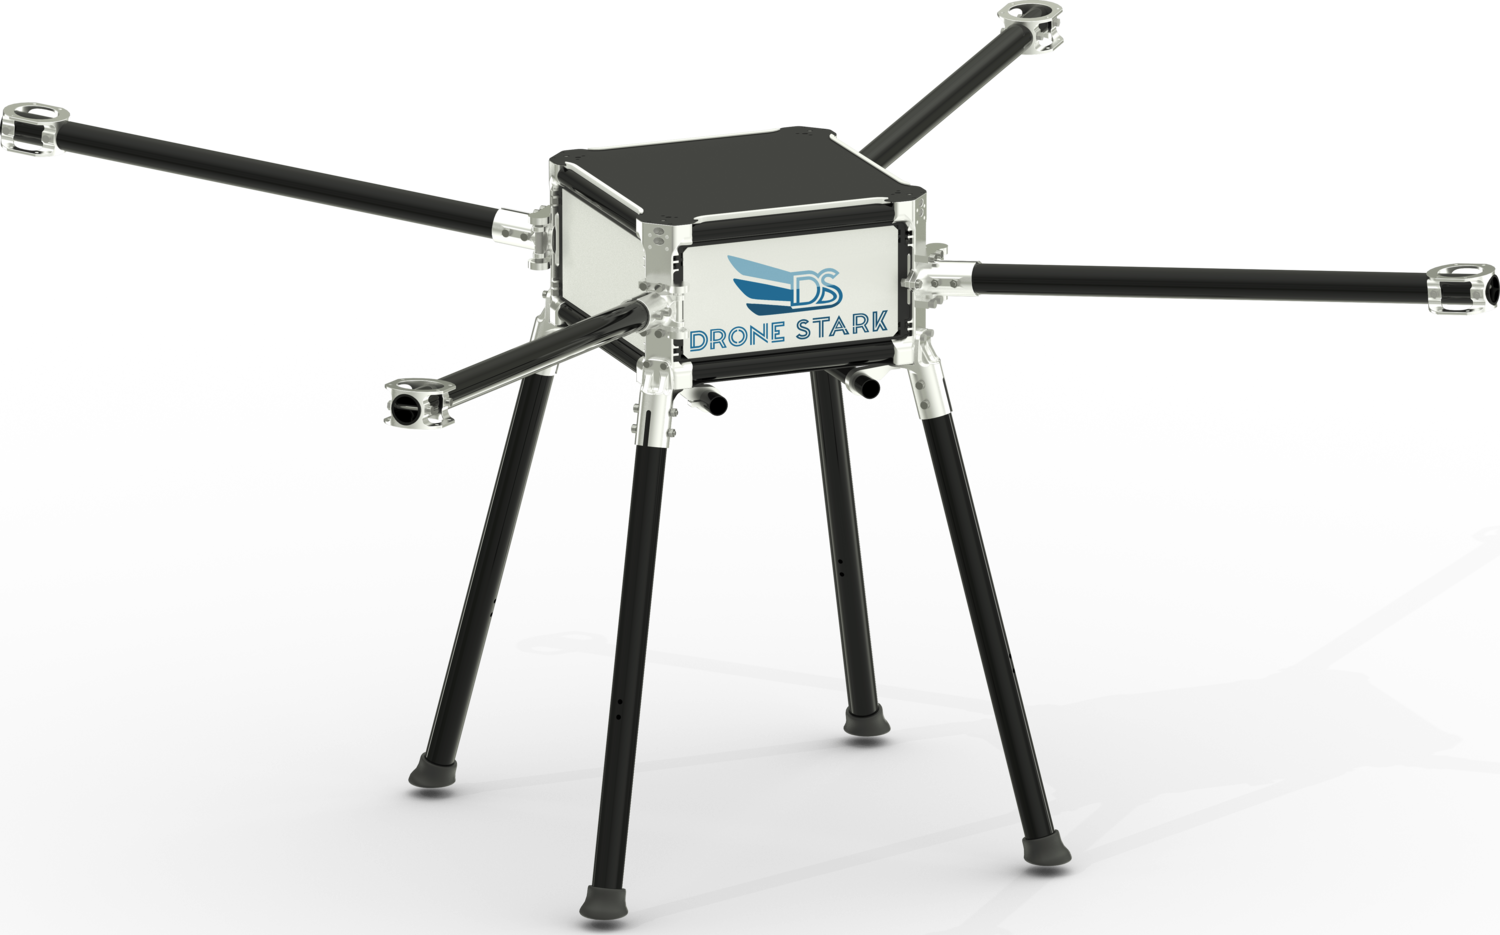
\includegraphics[width=\textwidth]{szl-dronestark-body.png}
        \caption{Frame}
        \label{fig:sfig-szl-body-frame}
    \end{subfigure}
    \begin{subfigure}[b]{0.3\textwidth}
        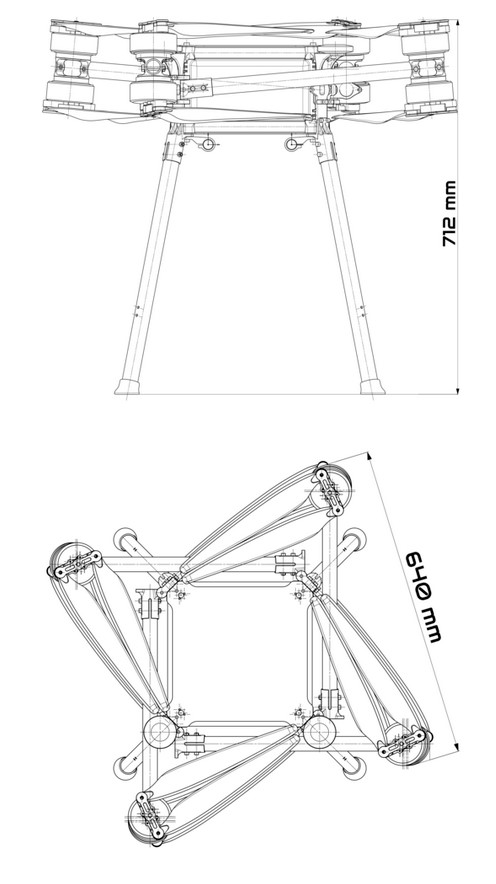
\includegraphics[width=\textwidth]{szl-dronestark-size-folded.jpg}
        \caption{Folded}
        \label{fig:sfig-szl-size-folded}
    \end{subfigure}
    \begin{subfigure}[b]{0.3\textwidth}
        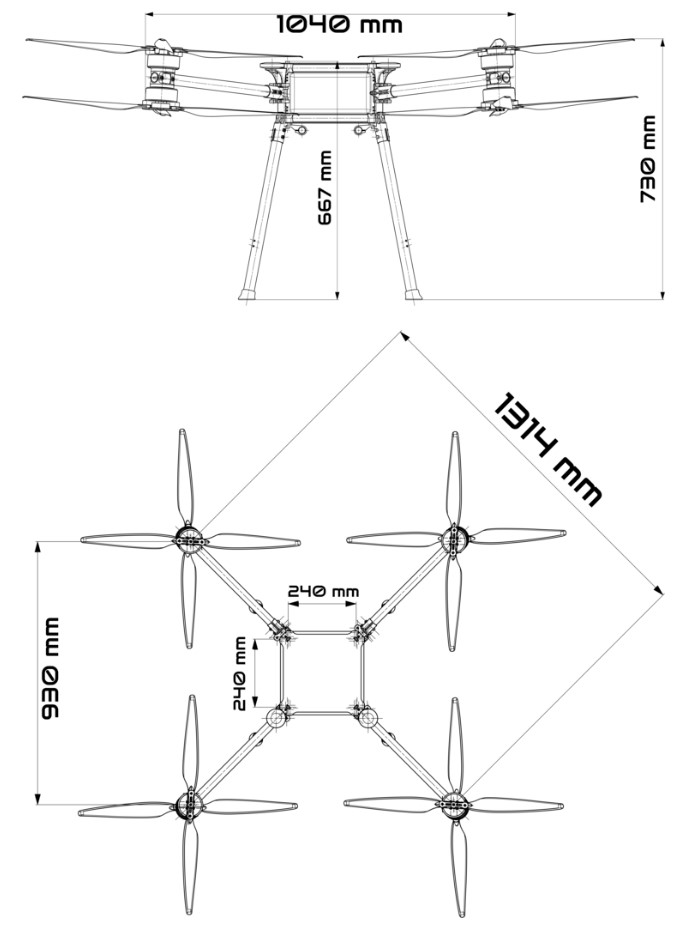
\includegraphics[width=\textwidth]{szl-dronestark-size-extended.jpg}
        \caption{Extended}
        \label{fig:sfig-szl-size-extended}
    \end{subfigure}
    \caption{Body and Dimensional Specifications}
    \label{fig:szl-body-specs}
    \small
        All figures are from \url{https://www.dronestark.com/octaglide}. The frame in \ref{sub@fig:sfig-szl-body-frame} is patented by DroneStark.
        % CEO of DroneStark: Rohan Raut (rohanraut92@gmail.com)
\end{figure}

\paragraph*{Propellers and Motors}
The propellers were identified to have a $30$ inch diameter (approximately). They can be assumed to be \emph{foldable} $30\times10$ propellers made of carbon fiber, shown in figure \ref{fig:sfig-szl-props-blades}. The drone motors must be BLDC motors (high speed, power efficient). An approximate model could be something like the YP6215A+ BLDC motor shown in figure \ref{fig:sfig-szl-bldc-motor}. These are selected merely by matching physical dimensions, and are shown in figure \ref{fig:szl-props-motor}.

\begin{figure}[ht]
    \centering
    \begin{subfigure}[b]{0.3\textwidth}
        \centering
        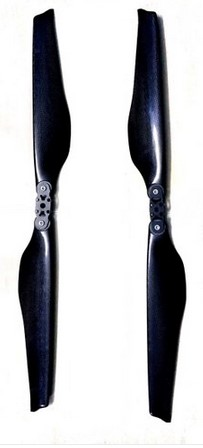
\includegraphics[width=\textwidth, height=2in, keepaspectratio]{szl-props-blades.jpg}
        \caption{Blades}
        \label{fig:sfig-szl-props-blades}
    \end{subfigure}
    \begin{subfigure}[b]{0.3\textwidth}
        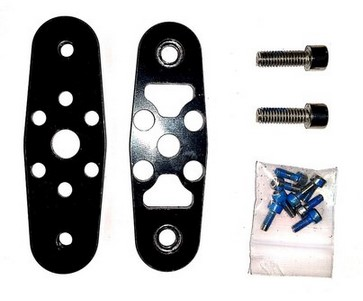
\includegraphics[width=\textwidth]{szl-props-hub-model.jpg}
        \caption{Hub}
        \label{fig:sfig-szl-props-hub}
    \end{subfigure}
    \begin{subfigure}[b]{0.3\textwidth}
        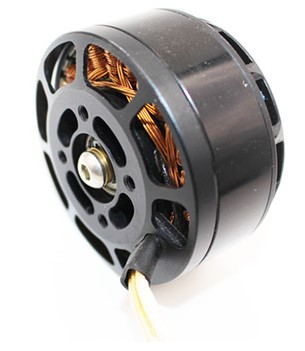
\includegraphics[width=\textwidth]{szl-bldc-cm.jpg}
        \caption{BLDC Motor}
        \label{fig:sfig-szl-bldc-motor}
    \end{subfigure}
    \caption{Propellers and BLDC Motor}
    \label{fig:szl-props-motor}
    \small
        Figure \ref{sub@fig:sfig-szl-props-blades} are of $30\times10$ propeller blades. They have $30$ inch diameter. The figure \ref{sub@fig:sfig-szl-props-hub} shows the hub which connects the two foldable parts of a blade.

        Figure \ref{sub@fig:sfig-szl-bldc-motor} is from \href{http://crazy-motor.com/pd.jsp?id=41#_pp=109_336}{crazy-motor}. Figures \ref{sub@fig:sfig-szl-props-blades} and \ref{sub@fig:sfig-szl-props-hub} are from \href{https://www.indiamart.com/proddetail/30-inch-foldable-carbon-fiber-propellers-21885512848.html}{indiamart}.
\end{figure}

\subsection{Component Identification}

Apart from the hardware components described above (for sizing and layout), the drone has the following components (described in paragraphs).

\begin{figure}[ht]
    \centering
    \begin{subfigure}[b]{0.3\textwidth}
        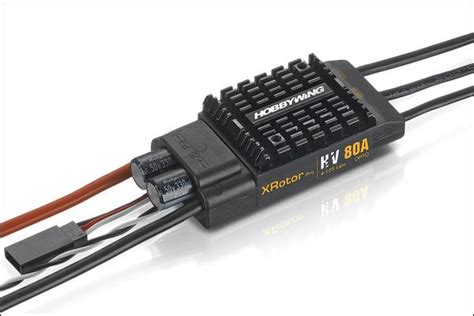
\includegraphics[width=\textwidth]{szl-esc.jpg}
        \caption{ESC}
        \label{fig:sfig-szl-esc-controller}
    \end{subfigure}
    \begin{subfigure}[b]{0.3\textwidth}
        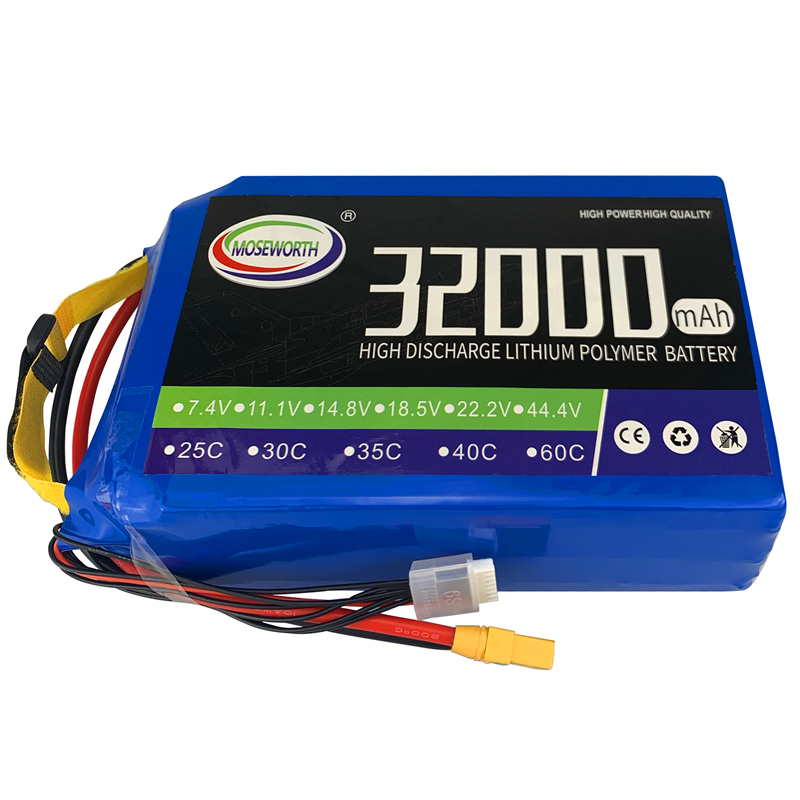
\includegraphics[width=\textwidth]{ci-battery.jpg}
        \caption{Battery}
        \label{fig:sfig-ci-battery}
    \end{subfigure}
    \begin{subfigure}[b]{0.3\textwidth}
        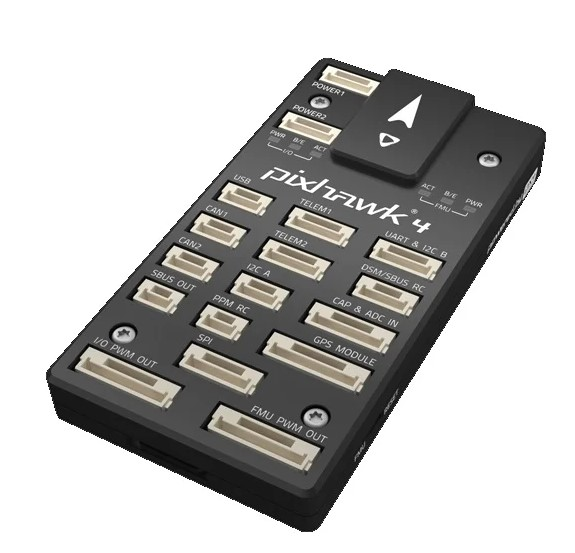
\includegraphics[width=\textwidth]{ci-fctrl.jpg}
        \caption{Controller}
        \label{fig:sfig-ci-fctrl}
    \end{subfigure}
    \caption{ESC, Battery and Controller}
    \label{fig:ci-esc-battery-ctrl}
    \small
        Figure \ref{sub@fig:sfig-szl-esc-controller} is from \href{https://www.hobbywingdirect.com/products/xrotor-pro-80a-hv-esc-dual-pack}{hobbywingdirect}.
        Figure \ref{sub@fig:sfig-ci-battery} is from \href{https://www.alibaba.com/product-detail/High-Performance-44-4V-32000mAh-25C_1600101213026.html}{MouseWorth on Alibaba}.
        Figure \ref{sub@fig:sfig-ci-fctrl} is from \href{https://robu.in/product/holybro-original-pixhawk-px4-flight-controller-without-gps/}{robu.in}.
\end{figure}

\paragraph*{ESC}
The ESC (Electronic Speed Controller) recommended by the motor manufacturer of the BLDC motor shown in figure \ref{fig:sfig-szl-bldc-motor} is an $80\,A$ HV (high voltage) ESC. A suitable model is \texttt{XRotor PRO 80A-HV ESC} shown in figure \ref{fig:sfig-szl-esc-controller}. Note that we will need eight of these controllers. We can theoretically use four (tap the wiring of the motors in the same branch), but that is not recommended.

\paragraph*{Battery}
The battery capacity listed in the \href{https://www.dronestark.com/octaglide}{OctaGlide specifications} is \texttt{32000 mAH / 1420 Watt-Hour}. This is the internal battery. The voltage is $V = \sfrac{1420\,Wh}{32\,Ah}=44.375\,V \approx 44.4\,V$. A battery with high enough C rating is needed \footnote{The C Rating gives an estimate of charging and discharging current of a battery $I = C_{r} \times E_{Ah}$. More \href{https://www.power-sonic.com/blog/what-is-a-battery-c-rating/}{here}}. We can choose the \texttt{MoseWorth 44.4V 32000mAh 25C 12S RC LiPo Battery}, as shown in figure \ref{fig:sfig-ci-battery}. The same battery can be used as an extra battery, mounted externally to extend the range of UAV. The battery size of $215, 134, 130\,mm$ should fit inside the body frame.

\paragraph*{Controller}
We can use the \texttt{Holybro Original Pixhawk PX4} Flight Controller. It has a redundant power supply inputs, microSD storage, an abundant power supply, and multiple additional peripherals for controlling IO. The processor is \texttt{STM32F76}. This controller is shown in figure \ref{fig:sfig-ci-fctrl}.

\subsubsection*{Additional payloads}

The following components are core to agricultural and regulatory compliance. Some sensors are also mentioned here.

\paragraph*{Payload: Tank, pump and spray}
The tank, stored on top of the body, is shown in figure \ref{fig:sfig-ci-agri-comps}. This tank stores the liquid fertilizer that is to be sprayed on the agricultural field. A pump (also included in figure \ref{fig:sfig-ci-agri-comps}) pushes the liquid from the tank to the spray nozzle.

\paragraph*{GPS and orientation sensors}
A GPS module is required for mapping (and regulatory compliance). A simple module that can be used is \texttt{Ublox NEO-M8N 7M GPS Module}. This is shown in figure \ref{fig:sfig-ci-gps}. It is a package that contains the \href{https://www.u-blox.com/en/product/neo-m8-series}{NEO-M8 series} GNSS module. An IMU (orientation sensors) is required for localizing and control. The \texttt{Adafruit 9-DOF IMU} is a good choice with \texttt{LSM303DLHC} (3-axis accelerometer and 3-axis magnetometer) and \texttt{L3GD20} (3-axis gyroscope) on the same board. This is shown in figure \ref{fig:sfig-ci-imu}. These sensors have to be connected to the controller shown in figure \ref{fig:sfig-szl-esc-controller}.

\paragraph*{Altimeter}
The altimeter \texttt{Adafruit BMP388 and BMP390} can be used for getting altitude data. This can be found \href{https://learn.adafruit.com/adafruit-bmp388-bmp390-bmp3xx/arduino}{here}. A kind of encoder might be needed to connect with the flight controller.

\begin{figure}
    \centering
    \begin{subfigure}[b]{0.475\textwidth}
        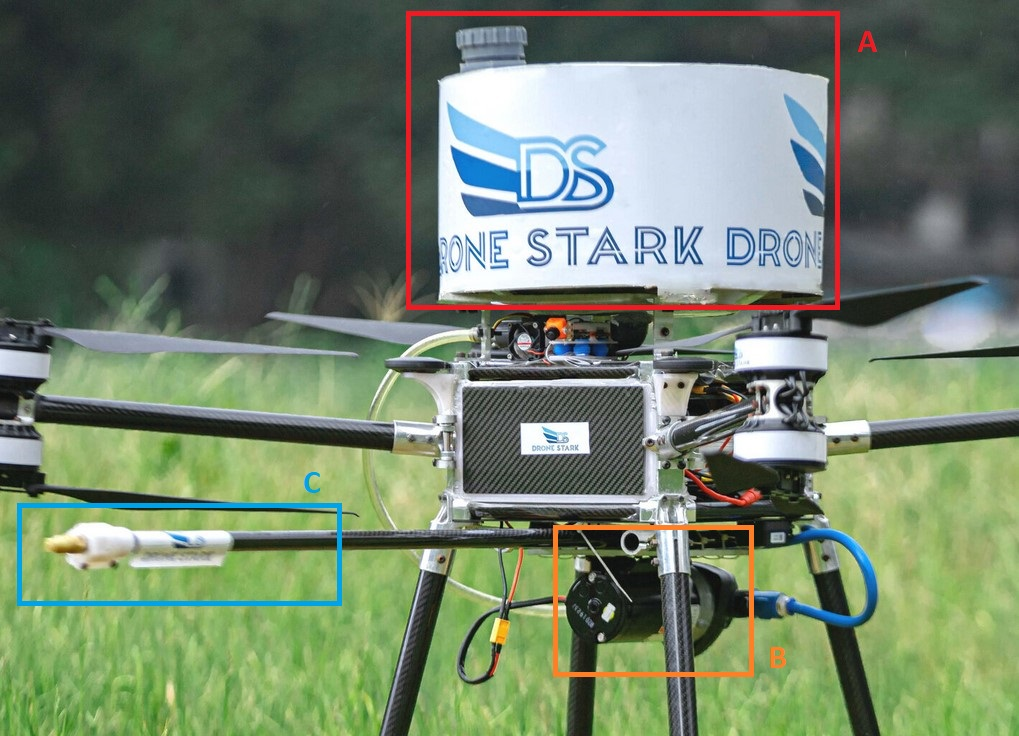
\includegraphics[width=\textwidth]{ci-agri-components-ann.jpg}
        \caption{Payload}
        \label{fig:sfig-ci-agri-comps}
    \end{subfigure}
    \begin{subfigure}[b]{0.249\textwidth}
        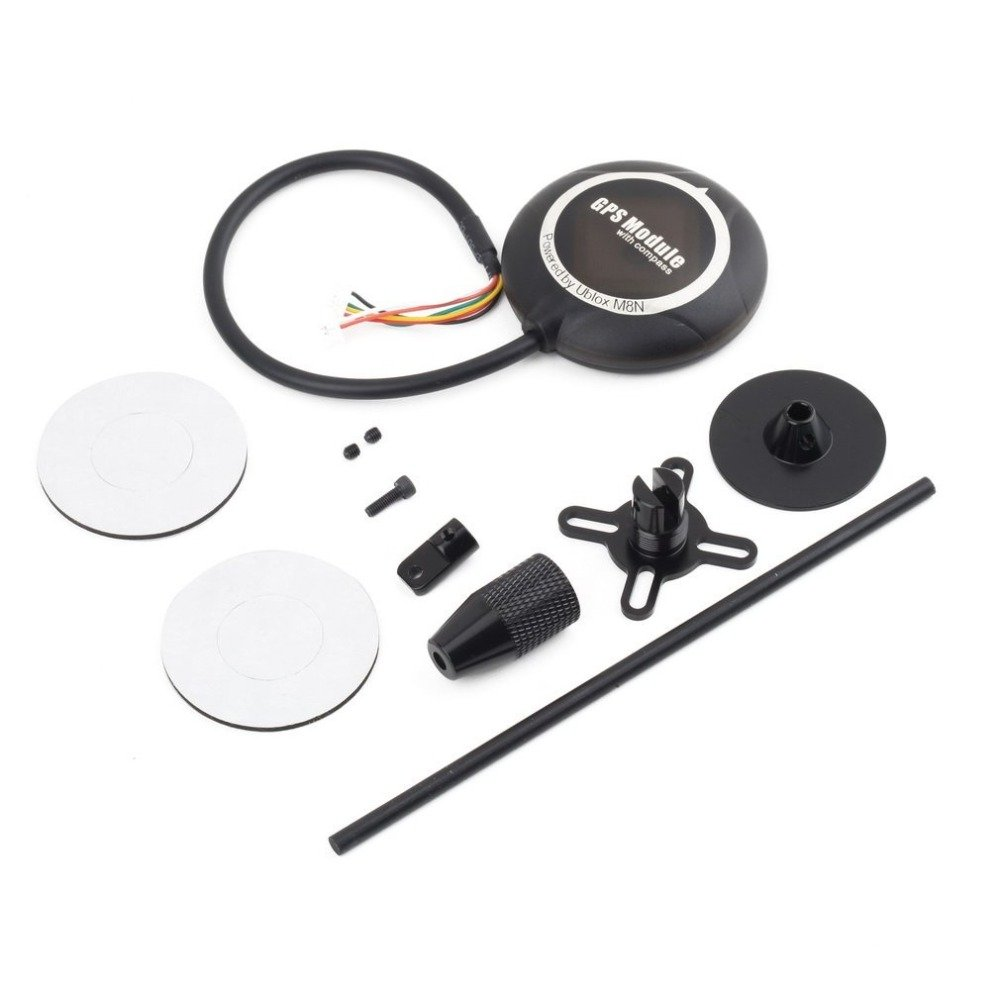
\includegraphics[width=\textwidth]{ci-gps.jpg}
        \caption{GPS}
        \label{fig:sfig-ci-gps}
    \end{subfigure}
    \begin{subfigure}[b]{0.249\textwidth}
        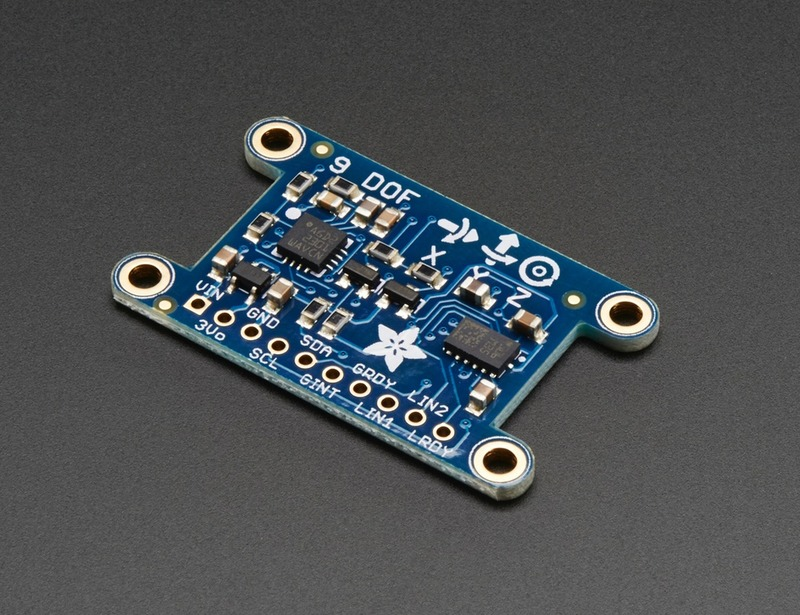
\includegraphics[width=\textwidth]{ci-agri-imu.jpg}
        \caption{IMU}
        \label{fig:sfig-ci-imu}
    \end{subfigure}
    \caption{Payloads}
    \small
        In \ref{sub@fig:sfig-ci-agri-comps}, the component \texttt{A} is the storage container for fertilizer. The component \texttt{B} is the pump for pumping that liquid fertilizer to the nozzle spray. The component \texttt{C} is the spray nozzle which uniformly sprays the fertilizer.

        Figure \ref{sub@fig:sfig-ci-agri-comps} is from \href{https://www.dronestark.com/octaglide}{dronestark} website. Figure \ref{sub@fig:sfig-ci-gps} is from \href{https://www.amazon.in/dp/B06Y2D1F41/ref=cm_sw_em_r_mt_dp_WF3X2SMNF0ES421ECGB4}{Amazon}. Figure \ref{sub@fig:sfig-ci-imu} is from \href{https://learn.adafruit.com/adafruit-9-dof-imu-breakout}{adafruit}.
\end{figure}
